\documentclass[border=4pt]{standalone}
\usepackage{tikz}
\usetikzlibrary{positioning, arrows.meta, shapes.geometric, calc, fit, backgrounds, decorations.pathreplacing}
\usepackage{amsmath,amssymb}
\begin{document}
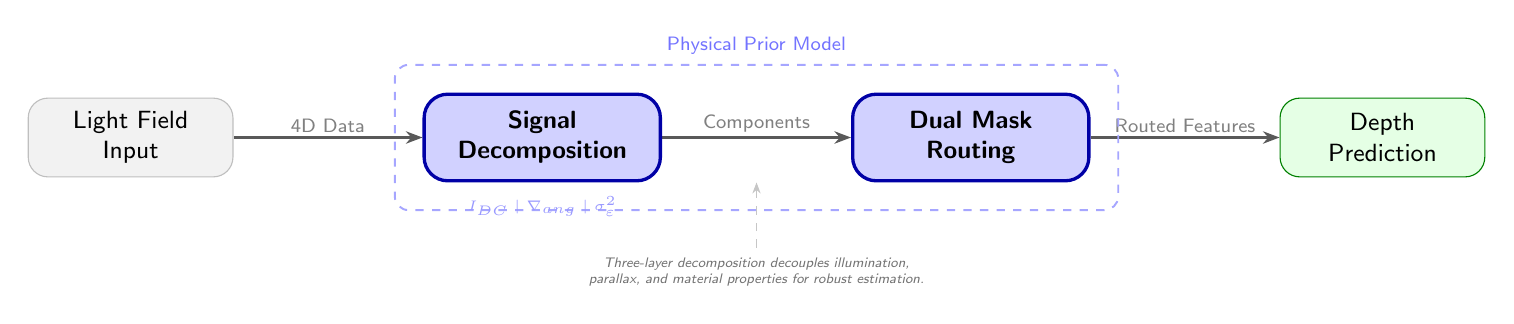
\begin{tikzpicture}[
  input/.style={draw, rounded corners=2.5mm, minimum width=2.6cm, minimum height=1.0cm,
                fill=gray!10, draw=gray!50, align=center, font=\sffamily\small},
  innov/.style={draw, rounded corners=3mm, minimum width=3.0cm, minimum height=1.1cm,
                fill=blue!18, draw=blue!65!black, line width=1.2pt, align=center,
                font=\sffamily\small\bfseries},
  output/.style={draw, rounded corners=2.5mm, minimum width=2.6cm, minimum height=1.0cm,
                 fill=green!10, draw=green!50!black, align=center, font=\sffamily\small},
  arr/.style={-{Stealth[length=6pt]}, thick, color=black!65},
  lbl/.style={font=\sffamily\scriptsize, text=black!50, fill=white, inner sep=1.5pt},
  gbox/.style={draw=blue!35, dashed, rounded corners=5pt, inner sep=10pt, line width=0.7pt},
  annotation/.style={font=\sffamily\tiny\itshape, text=black!55, align=center},
]

% === Nodes (main layer) ===
\node[input] (m1) {Light Field\\Input};

\node[innov, right=2.4cm of m1] (m2) {Signal\\Decomposition};

\node[innov, right=2.4cm of m2] (m3) {Dual Mask\\Routing};

\node[output, right=2.4cm of m3] (m4) {Depth\\Prediction};

% === Annotation callout below the group ===
\node[annotation, below=1.4cm of $(m2)!0.5!(m3)$, text width=7cm] (note)
  {Three-layer decomposition decouples illumination,\\
   parallax, and material properties for robust estimation.};

% === Arrows (background layer) ===
\begin{pgfonlayer}{background}
  % Main data flow
  \draw[arr] (m1) -- node[lbl, above] {4D Data} (m2);
  \draw[arr] (m2) -- node[lbl, above] {Components} (m3);
  \draw[arr] (m3) -- node[lbl, above] {Routed Features} (m4);

  % Annotation connector (dashed, subtle)
  \draw[-{Stealth[length=4pt]}, dashed, color=gray!45]
    (note.north) -- ($(m2.south)!0.5!(m3.south)$);

  % Group box around innovation modules
  \node[gbox, fit=(m2)(m3),
        label={[font=\sffamily\scriptsize, text=blue!55]above:Physical Prior Model}] (g1) {};
\end{pgfonlayer}

% === Small visual detail: sub-decomposition hints inside m2 ===
\node[font=\sffamily\tiny, text=blue!40, below=0.05cm of m2.south, anchor=north]
  {$I_{DC}\;|\;\nabla_{ang}\;|\;\sigma^2_{\varepsilon}$};

\end{tikzpicture}
\end{document}